% GitHub Desktop 的简单使用
% 代码管理|Github|git|Github Desktop

\subsection{Git 与 GitHub}
要了解 GitHub 首先要了解 Git. Git 是一个文件版本控制程序, 通常用于管理程序代码, 但也可以用来管理任何文件. 从某种意义上来讲, Git 相当于一个强大的备份软件, 它可以保存一个文件夹内所有子文件夹和文件(这个文件夹叫做 \textbf{仓库(repository)}, 简称 \textbf{repo})的许多不同时间的 \textbf{snapshot}(快照, 即所有文件某时刻的内容),而且可以对比出每个快 snapshot 相对上一个的变化. 但查看变化仅限文本文档, 但 word 和 pdf 可以通过插件先自动转换为文本文档再做对比. Git 还可以给文件夹创造不同的 \textbf{branch (分支)}, 例如一个程序写到一定的阶段后, 我们希望将其向两个不同的方向发展为两个功能略不相同的程序,就可以创建一个新的分支, 分别记录这两个程序的发展.

Git 本身是一个基于控制行的程序, 最初是为了管理 Linux 操作系统的源代码而创造的, 虽然 Git 现在已经有了各种各样的图形界面程序, 但控制行版本的功能仍然是最齐全的. 所以一般的 Git 教程都是控制行版本的教程. 这里不介绍控制行\footnote{可以参考\href{https://git-scm.com/book/en/v2}{官方教程}.}, 而是介绍一个简单但广泛使用的界面程序 GitHub Desktop, 注意该程序只能在 Windows 或 Mac 系统中安装.

Git 的一个重要功能就是可以让许多人合作完成一个工程, 这个功能通常需要在一台服务器中安装 Git Server, 每个合作者加入时把服务器中的 repo \textbf{clone}(克隆)到自己的电脑上. 更常见地是使用一些提供 server 的网站, 如 \href{https://github.com}{github.com}. 通过 Git 或者 GitHub Desktop 也可以把 github.com 上的开源项目 clone 到本地.

Git 中的每一个快照也叫 \textbf{commit}, 都是通过手动\textbf{提交(commit)} 操作完成. 我们可以随时查看当前文件夹中的文件与上次 commit 相比是否发生了改动, 以及改动了什么内容, 也可以选择撤销哪些改动.
 
\subsection{创建第一个仓库}
在\href{https://desktop.github.com/}{官网}下载 GitHub Desktop 并安装打开, 可以登录或注册 GitHub 账号. 注意 GitHub Enterprise 是企业账号, 个人账号是免费注册的. 注意免费账号只能建立 public repo(任何人都能访问或下载), 创建私密的的 private repo 需要开通会员. 目前使用 edu 结尾的学生邮箱注册可以获得免费会员.

\begin{figure}[ht]
\centering
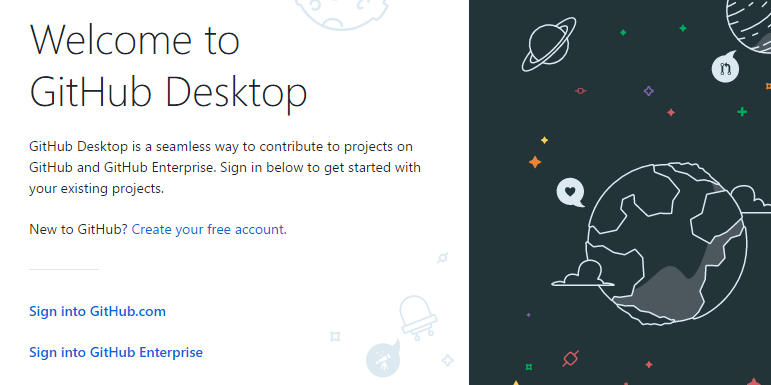
\includegraphics[width=13cm]{./figures/GitHub_1.png}
\caption{GitHub Desktop 登录} \label{GitHub_fig1}
\end{figure}

登录以后可以选择新建一个 repo 或者从 github 上 clone, 我们这里选择新建(如\autoref{GitHub_fig2}). 根据提示输入 repo 的名称 \lstinline|test|, 描述 \lstinline|learn to use GitHub Desktop|, 文件夹储存目录(默认是 \lstinline|Documents/GitHub/|). 勾选 Initialize this repository with a README. 然后就可以确定了.

\begin{figure}[ht]
\centering
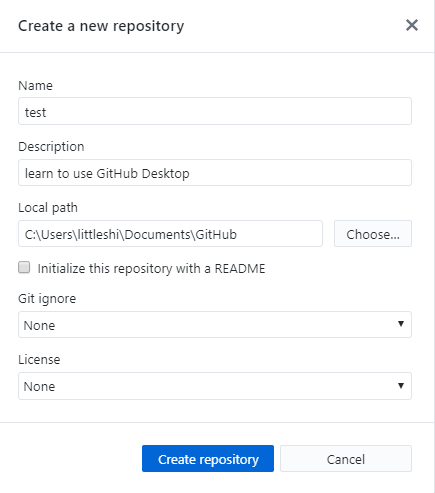
\includegraphics[width=8cm]{./figures/GitHub_3.png}
\caption{新建仓库} \label{GitHub_fig2}
\end{figure}

创建完后界面如\autoref{GitHub_fig3} 所示
\begin{figure}[ht]
\centering
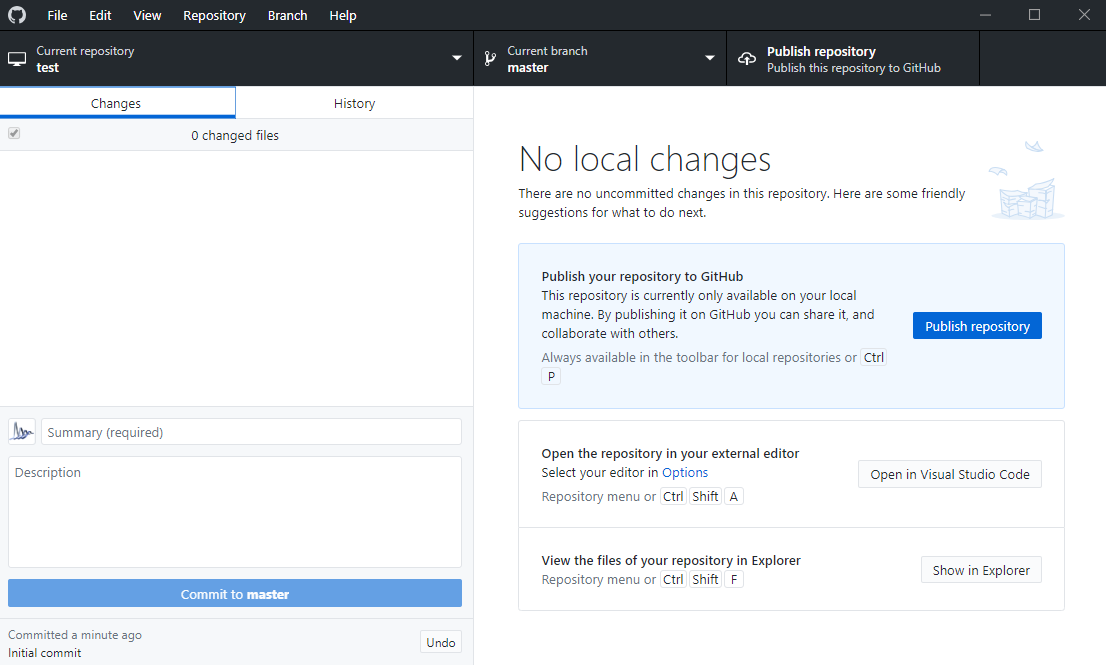
\includegraphics[width=15cm]{./figures/GitHub_4.png}
\caption{repo 主界面} \label{GitHub_fig3}
\end{figure}

单击 History 可以看到左下角已经有一个 Initial commit 了, 所有的 commit 的历史可以在左上角的 History 找到. 点击 History 可以看到 Initial commit 中添加了两个文件, \lstinline|README.md| 和 \lstinline|.gitattributes|. 其中 \lstinline|README.md| 是一个文本文档, 可以添加 repo 的描述, 使用说明等. \lstinline|.gitattributes| 文件用于对 Git 做一些设置, 例如如何处理换行\footnote{Windows 系统的换行使用 CR 和 LF 两个字符, 而 Linux 系统中只用一个 LF 字符.}. 如果新建 repo 的时候没有勾选 Initialize this repository with a README, 就不会有 Initial commit. 点击左上角的 Changes 返回刚才的界面.

注意左下角有一个 Undo 按钮. 如果按下, Initial commit 将被撤销. 再来看右上角的 Push 按钮, 这个按钮用于把新增的 commit 上传(即 push)到 GitHub. 由于我们从来没有 push 过, 现在打开 GitHub 网站是看不到刚刚创建的项目的. 按下 push, 完成后再刷新浏览器就可以在 GitHub 看到了.
\begin{figure}[ht]
\centering
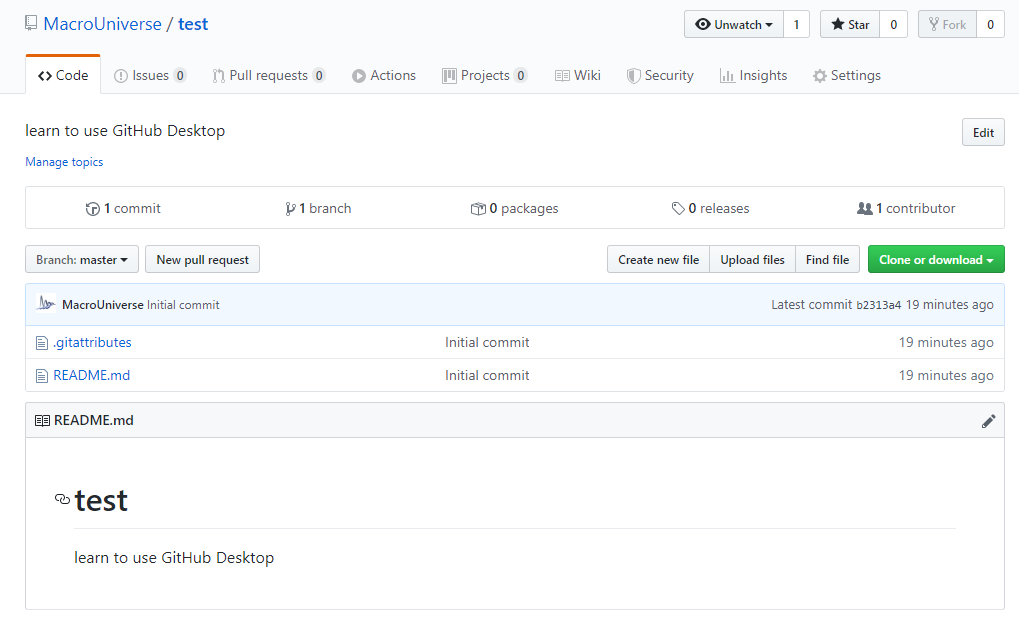
\includegraphics[width=15cm]{./figures/GitHub_5.png}
\caption{GitHub 网站上查看 repo} \label{GitHub_fig5}
\end{figure}

\subsection{Commit}
